\begin{frame}
    \frametitle{CUDA}
    \framesubtitle{Introduction}
    \begin{itemize}
        \item 
    \end{itemize}
\end{frame}

\begin{frame}
    \frametitle{CUDA}
    \framesubtitle{Program structure}
    \begin{figure}
        \centering
        \label{fig:cuda-structure}
        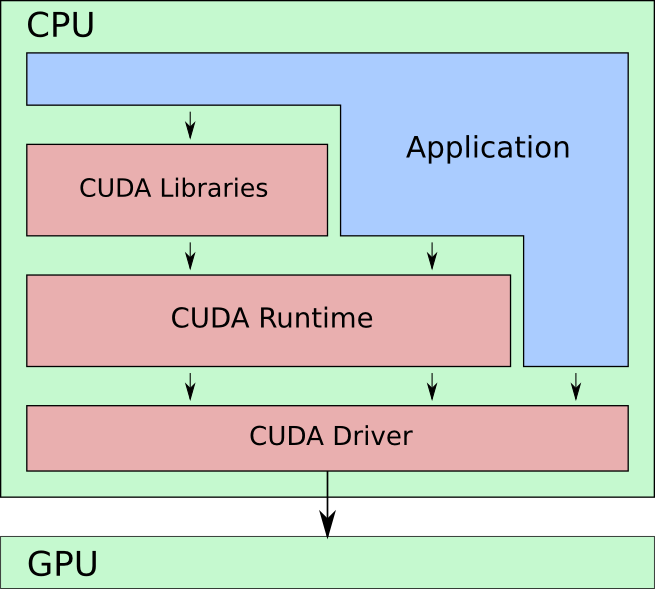
\includegraphics[width=0.5\textwidth]{img/cuda-structure}
        \caption{Program structure}
    \end{figure}
\end{frame}

\begin{frame}
    \frametitle{CUDA}
    \framesubtitle{Program structure - Example}

    ...
\end{frame}



\begin{frame}
    \frametitle{CUDA}
    \framesubtitle{Threads and blocks}
    \begin{itemize}
        \item 
    \end{itemize}
\end{frame}

\begin{frame}
    \frametitle{CUDA}
    \framesubtitle{Memories}
    \begin{figure}
        \centering
        \label{fig:cuda-memories}
        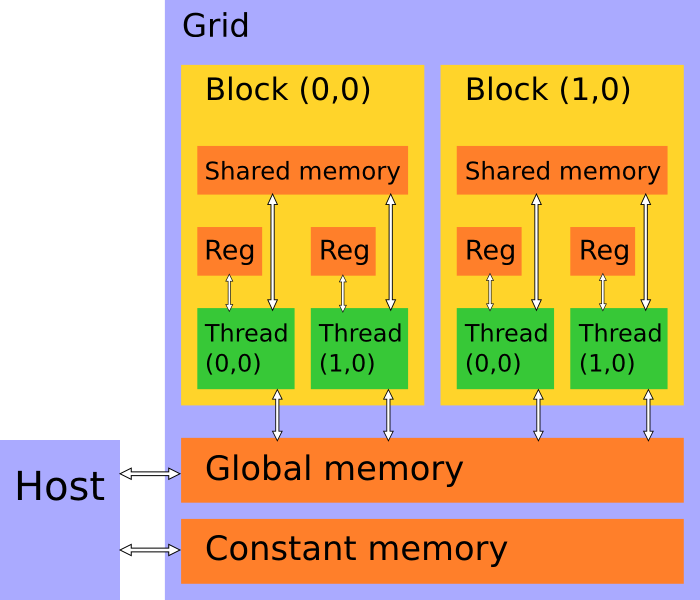
\includegraphics[width=0.5\textwidth]{img/cuda-memories}
        \caption{GPU Memories}
    \end{figure}
\end{frame}

\begin{frame}[fragile]
    \frametitle{CUDA}
    \framesubtitle{Memories}
    \begin{table}
    \centering
    \label{tab:memories-penalty}
    \scriptsize
    \begin{tabular}{l|r|r|r|r}
        \textbf{Declaration}  & \textbf{Memory}   & \textbf{Scope}  & \textbf{Lifetime}    & \textbf{Penalization} \\
        \texttt{int var;}                      & Register & Thread & Thread      & 1x \\
        \texttt{int a\_var[10];}            & Local    & Thread & Thread      & 100x \\
        \texttt{\_\_shared\_\_ int sh\_var;}    & Shared   & Block  & Block       & 1x \\
        \texttt{\_\_device\_\_ int gl\_var;}    & Global   & Grid   & Application & 100x \\
        \texttt{\_\_constant\_\_ int ct\_var;}& Constant & Grid   & Application & 1x 
    \end{tabular}
    \label{CUDA Memories}
    \end{table}
\end{frame}

\begin{frame}
    \frametitle{CUDA}
    \framesubtitle{Memories - Example}

    ...
\end{frame}

\begin{frame}
    \frametitle{CUDA}
    \framesubtitle{Programming strategy}
    \begin{figure}
        \centering
        \label{fig:cuda-strategy}
        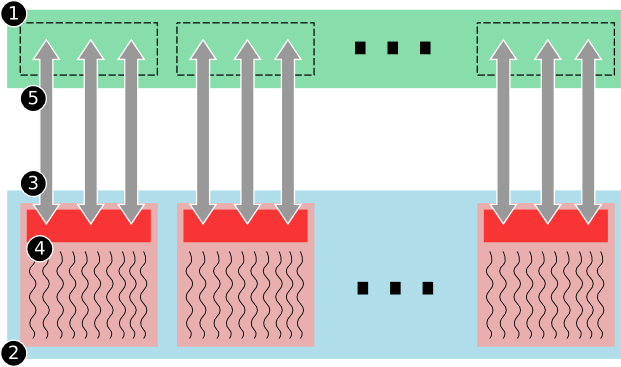
\includegraphics[width=0.6\textwidth]{img/cuda-strategy}
        \caption{GPU programming strategy}
    \end{figure}
\end{frame}

\begin{frame}
    \frametitle{CUDA}
    \framesubtitle{Programming strategy - Example}
    ...
\end{frame}
